\documentclass[11pt,                    % corpo del font principale
               a4paper,                 % carta A4
               twoside,                 % impagina per fronte-retro
               openright,               % inizio capitoli a destra
               english,
               italian,
               ]{book}

\usepackage[utf8]{inputenc}
\usepackage[english, italian]{babel}
\usepackage{graphicx}                   % immagini
\usepackage{listings}
\usepackage{color}
\usepackage{xcolor}
\definecolor{mygreen}{rgb}{0,0.5,0}
\lstnewenvironment{codice_json}[1][]
{\lstset{basicstyle=\small\ttfamily, columns=fullflexible,
keywordstyle=\color{green}\bfseries, commentstyle=\color{violet}, stringstyle=\color{blue},
language=Java, frame=single}}{}
\lstnewenvironment{codice_java}[1][]
{\lstset{basicstyle=\small\ttfamily, columns=fullflexible,
keywordstyle=\color{blue}\bfseries, commentstyle=\color{mygreen}, stringstyle=\color{violet},
language=Java, breaklines=true, breakatwhitespace=true,
frame=single, morekeywords={*,EventBus,VertxOptions,EventBusOptions}}}{}
\usepackage{hyperref}
%**************************************************************
% file contenente le impostazioni della tesi
%**************************************************************

%**************************************************************
% Frontespizio
%**************************************************************

% Autore
\newcommand{\myName}{Simone Barco}
\newcommand{\myTitle}{Piattaforma di video streaming per assistenza da remoto su dispositivi wearable}

% Tipo di tesi
\newcommand{\myDegree}{Tesi di laurea triennale}

% Università
\newcommand{\myUni}{Università degli Studi di Padova}

% Facoltà
\newcommand{\myFaculty}{Corso di Laurea in Informatica}

% Dipartimento
\newcommand{\myDepartment}{Dipartimento di Matematica "Tullio Levi-Civita"}

% Titolo del relatore
\newcommand{\profTitle}{Prof.}

% Relatore
\newcommand{\myProf}{Gilberto Filè}

% Luogo
\newcommand{\myLocation}{Padova}

% Anno accademico
\newcommand{\myAA}{2017-2018}

% Data discussione
\newcommand{\myTime}{Febbraio 2018}


%**************************************************************
% Impostazioni di impaginazione
% see: http://wwwcdf.pd.infn.it/AppuntiLinux/a2547.htm
%**************************************************************

\setlength{\parindent}{14pt}   % larghezza rientro della prima riga
\setlength{\parskip}{0pt}   % distanza tra i paragrafi


%**************************************************************
% Impostazioni di biblatex
%**************************************************************
% \bibliography{bibliografia} % database di biblatex
%
% \defbibheading{bibliography} {
%     \cleardoublepage
%     \phantomsection
%     \addcontentsline{toc}{chapter}{\bibname}
%     \chapter*{\bibname\markboth{\bibname}{\bibname}}
% }
%
% \setlength\bibitemsep{1.5\itemsep} % spazio tra entry
%
% \DeclareBibliographyCategory{opere}
% \DeclareBibliographyCategory{web}
%
% \addtocategory{opere}{womak:lean-thinking}
% \addtocategory{web}{site:agile-manifesto}
%
% \defbibheading{opere}{\section*{Riferimenti bibliografici}}
% \defbibheading{web}{\section*{Siti Web consultati}}
%
%
% %**************************************************************
% % Impostazioni di caption
% %**************************************************************
% \captionsetup{
%     tableposition=top,
%     figureposition=bottom,
%     font=small,
%     format=hang,
%     labelfont=bf
% }
%
% %**************************************************************
% % Impostazioni di glossaries
% %**************************************************************
% \input{gloss.tex} % database di termini
% \makeglossaries


%**************************************************************
% Impostazioni di graphicx
%**************************************************************
\graphicspath{{immagini/}} % cartella dove sono riposte le immagini


%**************************************************************
% Impostazioni di hyperref
%**************************************************************
\hypersetup{
    linktoc=all,
    colorlinks=true,
    linkcolor=black,
    urlcolor=black
}

  %   prima
  % colorlinks=true,
  % linktocpage=black,
  % linkcolor=blue,
  % urlcolor=blue
    %hyperfootnotes=false,
    %pdfpagelabels,
    %draft,	% = elimina tutti i link (utile per stampe in bianco e nero)
    % colorlinks=true,
    % linktocpage=true,
    % pdfstartpage=1,
    % pdfstartview=FitV,
    % % decommenta la riga seguente per avere link in nero (per esempio per la stampa in bianco e nero)
    % %colorlinks=false, linktocpage=false, pdfborder={0 0 0}, pdfstartpage=1, pdfstartview=FitV,
    % breaklinks=true,
    % pdfpagemode=UseNone,
    % pageanchor=true,
    % pdfpagemode=UseOutlines,
    % plainpages=false,
    % bookmarksnumbered,
    % bookmarksopen=true,
    % bookmarksopenlevel=1,
    % hypertexnames=true,
    % pdfhighlight=/O,
    % %nesting=true,
    % %frenchlinks,
    % urlcolor=brown,
    % linkcolor=blue,
    % citecolor=green,
    % %pagecolor=RoyalBlue,
    % %urlcolor=Black, linkcolor=Black, citecolor=Black, %pagecolor=Black,
    % pdftitle={\myTitle},
    % pdfauthor={\textcopyright\ \myName, \myUni, \myFaculty},
    % pdfsubject={},
    % pdfkeywords={},
    % pdfcreator={pdfLaTeX},
    % pdfproducer={LaTeX}


%**************************************************************
% Impostazioni di itemize
%**************************************************************
%\renewcommand{\labelitemi}{$\ast$}

\renewcommand{\labelitemi}{$\bullet$}
%\renewcommand{\labelitemii}{$\cdot$}
%\renewcommand{\labelitemiii}{$\diamond$}
%\renewcommand{\labelitemiv}{$\ast$}


%**************************************************************
% Impostazioni di listings
%**************************************************************
% \lstset{
%     language=[LaTeX]Tex,%C++,
%     keywordstyle=\color{RoyalBlue}, %\bfseries,
%     basicstyle=\small\ttfamily,
%     %identifierstyle=\color{NavyBlue},
%     commentstyle=\color{Green}\ttfamily,
%     stringstyle=\rmfamily,
%     numbers=none, %left,%
%     numberstyle=\scriptsize, %\tiny
%     stepnumber=5,
%     numbersep=8pt,
%     showstringspaces=false,
%     breaklines=true,
%     frameround=ftff,
%     frame=single
% }


%**************************************************************
% Impostazioni di xcolor
%**************************************************************
% \definecolor{webgreen}{rgb}{0,.5,0}
% \definecolor{webbrown}{rgb}{.6,0,0}


%**************************************************************
% Altro
%**************************************************************

\newcommand{\omissis}{[\dots\negthinspace]} % produce [...]

% eccezioni all'algoritmo di sillabazione
\hyphenation
{
    ma-cro-istru-zio-ne
    gi-ral-din
}

\newcommand{\sectionname}{sezione}
\addto\captionsitalian{\renewcommand{\figurename}{Figura}
                       \renewcommand{\tablename}{Tabella}}

\newcommand{\glsfirstoccur}{\ap{{[g]}}}

\newcommand{\intro}[1]{\emph{\textsf{#1}}}

%**************************************************************
% Environment per ``rischi''
%**************************************************************
\newcounter{riskcounter}                % define a counter
\setcounter{riskcounter}{0}             % set the counter to some initial value

%%%% Parameters
% #1: Title
\newenvironment{risk}[1]{
    \refstepcounter{riskcounter}        % increment counter
    \par \noindent                      % start new paragraph
    \textbf{\arabic{riskcounter}. #1}   % display the title before the
                                        % content of the environment is displayed
}{
    \par\medskip
}

\newcommand{\riskname}{Rischio}

\newcommand{\riskdescription}[1]{\textbf{\\Descrizione:} #1.}

\newcommand{\risksolution}[1]{\textbf{\\Soluzione:} #1.}

%**************************************************************
% Environment per ``use case''
%**************************************************************
\newcounter{usecasecounter}             % define a counter
\setcounter{usecasecounter}{0}          % set the counter to some initial value

%%%% Parameters
% #1: ID
% #2: Nome
\newenvironment{usecase}[2]{
    \renewcommand{\theusecasecounter}{\usecasename #1}  % this is where the display of
                                                        % the counter is overwritten/modified
    \refstepcounter{usecasecounter}             % increment counter
    \vspace{10pt}
    \par \noindent                              % start new paragraph
    {\large \textbf{\usecasename #1: #2}}       % display the title before the
                                                % content of the environment is displayed
    \medskip
}{
    \medskip
}

\newcommand{\usecasename}{UC}

\newcommand{\usecaseactors}[1]{\textbf{\\Attori Principali:} #1. \vspace{4pt}}
\newcommand{\usecasepre}[1]{\textbf{\\Precondizioni:} #1. \vspace{4pt}}
\newcommand{\usecasedesc}[1]{\textbf{\\Descrizione:} #1. \vspace{4pt}}
\newcommand{\usecasepost}[1]{\textbf{\\Postcondizioni:} #1. \vspace{4pt}}
\newcommand{\usecasealt}[1]{\textbf{\\Scenario Alternativo:} #1. \vspace{4pt}}

%**************************************************************
% Environment per ``namespace description''
%**************************************************************

\newenvironment{namespacedesc}{
    \vspace{10pt}
    \par \noindent                              % start new paragraph
    \begin{description}
}{
    \end{description}
    \medskip
}

\newcommand{\classdesc}[2]{\item[\textbf{#1:}] #2}

\pagestyle{plain}
\begin{document}
  \frontmatter
  % !TEX encoding = UTF-8
% !TEX TS-program = pdflatex
% !TEX root = ../tesi.tex

%**************************************************************
% Frontespizio
%**************************************************************
\pagenumbering{gobble}% Remove page numbers (and reset to 1)
\thispagestyle{empty}
\begin{titlepage}

\begin{center}

\begin{LARGE}
\textbf{\myUni}\\
\end{LARGE}

\vspace{10pt}

\begin{Large}
\textsc{\myDepartment}\\
\end{Large}

\vspace{10pt}

\begin{large}
\textsc{\myFaculty}\\
\end{large}

\vspace{30pt}
\begin{figure}[htbp]
\begin{center}

\includegraphics[height=6cm]{logo-unipd}
\end{center}
\end{figure}
\vspace{30pt}

\begin{LARGE}
\begin{center}
\textbf{\myTitle}\\
\end{center}
\end{LARGE}

\vspace{10pt}

\begin{large}
\textsl{\myDegree}\\
\end{large}

\vspace{40pt}

\begin{flushleft}
  \textit{Relatore} \hfill \textit{Laureando}\\
  \vspace{5pt}
  \profTitle \myProf \hfill \myName
\end{flushleft}
% \begin{large}
% \begin{flushleft}
% \textit{Relatore}\\
% \vspace{5pt}
% \profTitle \myProf
% \end{flushleft}
%
% \vspace{0pt}
%
% \begin{flushright}
% \textit{Laureando}\\
% \vspace{5pt}
% \myName
% \end{flushright}
% \end{large}

\vspace{30pt}

\line(1, 0){338} \\
\begin{normalsize}
\textsc{Anno Accademico \myAA}
\end{normalsize}

\end{center}
\end{titlepage}

  % !TEX encoding = UTF-8
% !TEX TS-program = pdflatex
% !TEX root = ../tesi.tex

%**************************************************************
% Sommario
%**************************************************************
\cleardoublepage
\phantomsection
%\pdfbookmark{Sommario}{Sommario}
\begingroup
\let\clearpage\relax
\let\cleardoublepage\relax
\let\cleardoublepage\relax

\thispagestyle{empty}
\pagenumbering{gobble}% Remove page numbers (and reset to 1)

\thispagestyle{empty}
\chapter*{Sommario}

Il presente documento descrive l'esperienza di stage, svolto dal 23 Ottobre 2017 al 18 Dicembre 2017 dal laureando Simone Barco, presso l'azienda Vision Lab Apps S.R.L.\\
Lo scopo di questo stage era quello di studiare le componenti software già implementate e di  perseguire il loro miglioramento.\\
Queste componenti hanno lo scopo di realizzare una piattaforma di video streaming su dispositivi wearable per ottenere un'assistenza da remoto più performante.\\
Le principali tecnologie che sono state utilizzate sono Android e di conseguenza Java ed è stato studiato l'utilizzo di un toolkit che permette di migliorare la reattività di un sistema chiamato Vert.x.


%\vfill
%
%\selectlanguage{english}
%\pdfbookmark{Abstract}{Abstract}
%\chapter*{Abstract}
%
%\selectlanguage{italian}

\newpage
\null
\thispagestyle{empty}
\newpage

  % !TEX encoding = UTF-8
% !TEX TS-program = pdflatex
% !TEX root = ../tesi.tex

%**************************************************************
% Sommario
%**************************************************************
\cleardoublepage
\phantomsection
%\pdfbookmark{Sommario}{Sommario}
\begingroup
\let\clearpage\relax
\let\cleardoublepage\relax
\let\cleardoublepage\relax

\newpage
\thispagestyle{empty}
\pagenumbering{gobble}% Remove page numbers (and reset to 1)

\thispagestyle{empty}
\chapter*{Ringraziamenti}
\textit{Ringrazio innanzitutto i miei genitori per avermi supportato, e sopportato, durante tutto il percorso di studi.\\
Un grazie affettuoso alle mie nonne che mi hanno sempre aiutato, anche con un semplice chiacchierata per stemperare i momenti più difficili.\\
Un ringraziamento è dovuto anche a mio fratello Davide che, anche se non sempre poteva, ha cercato di stimolarmi a ragionare, ad usare la testa e portare a termine tutti i compiti che dovevo svolgere.\\
Un ringraziamento particolare va a una persona che non vuole essere nominata che però mi sento di fare perché, soprattutto nell'ultimo periodo, mi ha sopportato e spronato a fare meglio.\\
Infine un grazie a tutti gli amici e parenti per essere parte della mia vita, senza di loro non sarei arrivato fino a qui e non sarei la persona che sono.}
\begin{flushright}
  Simone Barco
\end{flushright}


%\vfill
%
%\selectlanguage{english}
%\pdfbookmark{Abstract}{Abstract}
%\chapter*{Abstract}
%
%\selectlanguage{italian}
\newpage
\null
\thispagestyle{empty}
\newpage

  \pagenumbering{Roman}
  % !TEX encoding = UTF-8
% !TEX TS-program = pdflatex
% !TEX root = ../tesi.tex

%**************************************************************
% Indici
%**************************************************************
\cleardoublepage
\pdfbookmark{\contentsname}{tableofcontents}
\setcounter{tocdepth}{2}
\tableofcontents
%\markboth{\contentsname}{\contentsname}
\clearpage
\newpage

\begingroup
    \let\clearpage\relax
    \let\cleardoublepage\relax
    \let\cleardoublepage\relax
    %*******************************************************
    % Elenco delle figure
    %*******************************************************
    \phantomsection
    \pdfbookmark{\listfigurename}{lof}
    \listoffigures

    \vspace*{8ex}
    \newpage
    \null
    \thispagestyle{empty}
    \newpage
    %*******************************************************
    % Elenco delle tabelle
    %*******************************************************
    % \phantomsection
    % \pdfbookmark{\listtablename}{lot}
    % \listoftables

    \vspace*{8ex}
\endgroup

\cleardoublepage


  \mainmatter
  % \hypersetup{
  %   linkcolor=blue
  % }

  
\chapter{Analisi del contesto aziendale}
\section{Vision Lab Apps e il suo ambito di attività}
  Vision Lab Apps S.R.L è una startup nata a New York nel 2011, con sede operativa a Torri di Quartesolo (VI), impegnata nel fornire servizi per la crescita del business delle \nameref{PMI}.
  I prodotti principalmente sviluppati dall'azienda sono \textit{software} personalizzati, siti web per il settore sanitario, manifatturiero e della sicurezza.\\
  È impegnata anche nello sviluppo di servizi \textit{cloud} e \textit{software} per dispositivi \nameref{Wear} e \nameref{IoT} in modo da permettere ai loro utenti di integrarsi in modo migliore con la rete di informazioni e sensori da cui sono circondati nella quotidianità.\\
  In particolare stanno eseguendo ricerca e sviluppo nel campo di visori per la realtà aumentata in modo da supportare le attività lavorative, promettendo grandi novità nel settore manifatturiero.
  \begin{figure}[h]
    \centering
    
\includegraphics[scale=0.3]{immagini/Logo-VLA-trasparente.png}
    \caption{Logo di Vision Lab Apps S.R.L}
    \label{logoVLA}
  \end{figure}
  \section{Progetti importanti}
    \subsubsection*{VisionHealthCare}
      VisionHealthCare è un \textit{software} prodotto da Vision Lab App in collaborazione con Dedalus S.P.A, società specializzata nello sviluppo di \textit{software} in ambito sanitario.
      Questa applicazione, che utilizza la suite applicativa web di Dedalus S.P.A chiamata OrmaWeb, utilizza gli occhiali per la realtà aumentata Google Glass per coprire tutte le azioni all'interno del percorso chirurgico.

      Si parte dalla gestione della lista d'attesa fino ad arrivare alla gestione del blocco operatorio, producendo anche il registro operatorio e la cartella anestesiologica prima e durante l'operazione.
      \begin{figure}[h]
        \centering
        
\includegraphics[scale=0.5]{immagini/vhc.png}
        \caption{Logo VisionHealthCare}
        \label{logoVHC}
      \end{figure}

      I Google Glass si interfacciano con un'applicazione installata nello smartphone e si collegano tramite questo ai servizi di OrmaWeb.\\
      Questi occhiali permettono di registrare, durante l'operazione, note vocali correlate da video e foto che sono utili alla documentazione dell'operazione ma anche per attività di ricerca e di insegnamento.\\
      Il sistema permette di automatizzare buona parte di procedure di verbalizzazione dell'intervento, trascrivendo il testo registrato e unendolo ai dati già presenti in OrmaWeb.\\
      Questa soluzione permette di lavorare a mani libere e allo stesso tempo di ricevere dati aggiuntivi sullo stato del paziente.
    \newpage
    \subsubsection*{NapkinForever - Pininfarina Segno}
      Vision Lab Apps collabora anche con NapkinForever, azienda italiana di penne e stilo di design che da poco ha raggiunto un accordo di collaborazione con Pininfarina.\\
      Ha realizzato una presentazione virtuale dell'impresa per il Paperworld 2017, la più grande fiera mondiale di prodotti per l'ufficio e strumenti di scrittura.\\
      Questo progetto consisteva nella simulazione virtuale dei prodotti proposti da NapkinForever, inseriti in scenografie ad hoc, fornendo informazioni su di essi.\\
      Le tecnologie utilizzate comprendevano l'utilizzo di uno smartphone in accoppiata con i Google Cardboard, un apparato di lenti montate su un telaio di cartone.
      L'utilizzo di \textit{hardware} fatto di materiali poveri permetteva di fornire una buona esperienza d'uso ad un prezzo competitivo.
      Attualmente stanno sviluppando il sito web della nuova linea di prodotti nata dalla collaborazione con Pininfarina, design house di fama internazionale.
      \begin{flushleft}
        \begin{figure}[h]
          \centering
          
\includegraphics[scale=0.15]{immagini/forever.png}
          \caption{Logo NapkinForever e del nuovo \textit{brand} in collaborazione con Pininfarina}
          \label{logoNapkin}
        \end{figure}
      \end{flushleft}
  \section{Premi e certificazioni}
    \subsubsection*{UniCredit Start Lab}
    Vision Lab Apps ha partecipato alla competizione tra startup UniCredit Start Lab 2017.
    Durante questo evento le aziende che vi hanno partecipato hanno proposto le loro idee innovative in vari ambiti.\\
    L'azienda è stata valutata e inserita tra le 10 finaliste, guadagnando un periodo di incubazione e accelerazione da parte di UniCredit a partire da Settembre 2017.
    \begin{figure}[h]
      \centering
      
\includegraphics[scale=0.5]{immagini/unicredit.png}
      \caption{Logo di UniCredit Start Lab}
      \label{logoUnicredit}
    \end{figure}
    \newpage
    \subsubsection*{CES 2018 - Consumer Elettronic Show}
      Come conseguenza del periodo di incubazione e accelerazione da parte di UniCredit, Vision Lab Apps ha potuto partecipare, dopo un periodo di selezione, all'evento CES 2018.\\
      Il CES (Consumer Elettronic Show) è la più grande fiera mondiale di tecnologia di consumo e parteciparvi è senza dubbio un trampolino di lancio per avere maggiore visibilità a livello internazionale.\\
      Durante questo evento di quattro giorni tenutosi a Las Vegas, un altro indice di successo è stata la partecipazione dell'azienda all'elevator pitch di TechStars, incubatore di startup famoso a livello internazionale, come una delle 10 migliori realtà presenti all'evento.
      \begin{figure}[h]
        \centering
        
\includegraphics[scale=0.3]{immagini/ces.png}
        \caption{Logo CES - Consumer Elettronic Show}
        \label{logoCes}
      \end{figure}
  \newpage
  \section{Organizzazione aziendale}
    \subsection{Modello di sviluppo}
      Vision Lab Apps lavora con un metodo di sviluppo \textit{Agile} di tipo \textit{Scrum}.\\
      Questo modello si basa su principi fondamentali per svincolarsi da eccessiva rigidità. I principi fondamentali sono:
      \begin{itemize}
        \item le persone e le interazioni sono più importanti rispetto ai processi e agli strumenti;
        \item è molto più importante il \textit{software} rispetto alla documentazione;
        \item è molto più importante rispondere al cambiamento rispetto all'agire secondo un piano.
      \end{itemize}
      Questo pone una minore rigidità sulla documentazione e sulle formalità del prodotto, permettendo le modifiche in corso d'opera e maggiore flessibilità ai cambiamenti.\\
      Il metodo consiste nel fissare dei periodi di tempo brevi, gli \nameref{Sprint}, in cui vengono eseguite delle attività dette \nameref{Task}.\\
      In ogni \nameref{Sprint} il \textit{team} decide che \nameref{Task} eseguire e a chi vengono assegnati, prendendoli da un insieme organizzato detto \textit{backlog} del prodotto. In questo modo viene a crearsi un altro insieme organizzato di \nameref{Task} detto \textit{backlog} dello \nameref{Sprint}.\\
      Ogni giorno il \textit{team} si ritrova per una breve riunione in cui viene controllato lo stato dei vari \nameref{Task} o se sono sorte problematiche nella loro esecuzione, il \textit{daily scrum}.\\
      Al completamento di tutti i \nameref{Task} e quindi alla fine dello \nameref{Sprint} viene fatta un'ulteriore riunione in cui vengono discussi i problemi incontrati nell'esecuzione dei \nameref{Task}, discutendo inoltre quali precauzioni prendere per incorrere nuovamente nelle stesse complicazioni.\\\\
      Trattandosi di un metodo \textit{Agile} la documentazione è molto ridotta e quindi nasce il concetto di user story, documento fondamentale che contiene le richieste del cliente e le decisioni prese con lo stesso durante un incontro faccia a faccia.\\
      La presenza simultanea del cliente e di almeno un membro del \textit{team} permette una maggiore trasparenza e chiarezza riguardo le richieste del consumatore.\\
      Questo favorisce, inoltre, un'implementazione più semplice e diretta degli obiettivi da raggiungere.
      \newpage
      Per coordinamento del lavoro, l'assegnazione dei \nameref{Task} e il controllo dello stato degli stessi, l'azienda utilizza un applicazione web, Kanboard, che permette la creazione dei \nameref{Task}, la sua assegnazione con scadenze e le priorità.
      Tutto questa in una grafica che dà l'idea di una lavagna con dei post-it che possono essere spostati in base allo stato del \nameref{Task}.
      \begin{figure}[h]
        \centering
        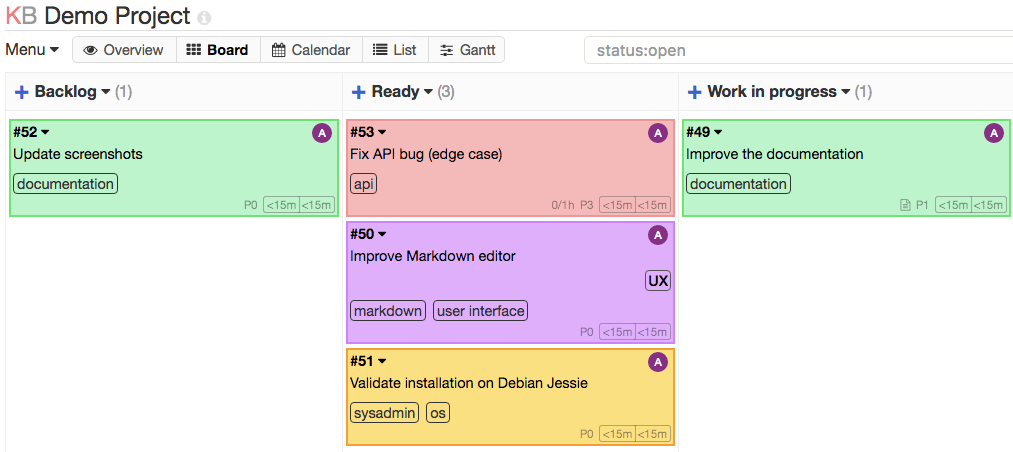
\includegraphics[scale=0.3]{immagini/board.png}
        \caption{Esempio della grafica di Kanboard}
        \label{kan}
      \end{figure}\\
      Questa applicazione web, visualizzabile da tutti i membri del \textit{team}, permette di avere una visione comune.\\
      Inoltre permette al \nameref{PM} di comprende le tempistiche di sviluppo per eventualmente capire come verrebbe gestita, a livello temporale, l'aggiunta di nuovi \nameref{Task} fornendo cioè una visione generale dell'utilizzo delle risorse.
    \subsection{Comunicazione}
      Per comunicare i membri del \textit{team} usano Slack, uno strumento di collaborazione aziendale che permette di inviare messaggi in modo istantaneo ai membri del \textit{team}.\\
      Inoltre viene usato anche Google Hangouts e Skype per permettere comunicazioni a distanza nel caso non fosse possibile riunire tutti i membri del \textit{team} nello stesso posto.
  \section{Tecnologie utilizzate dall'azienda}
    \subsection{Firebase}
      Firebase è una piattaforma di sviluppo per applicazioni web e \textit{mobile}, parte di Google Cloud Platform; fornisce servizi di scambio messaggi e basi di dati in tempo reale, spazio di archiviazione, sistemi di autenticazione, web \textit{hosting} e \textit{test} automatici per applicazioni Android.\\
      La piattaforma fornisce anche un servizio di analisi e profilazione degli utenti ed è presente anche l'integrazione con il sistema di annunci pubblicitari di Google.
      \begin{figure}[h]
        \centering
        
\includegraphics[scale=0.2]{immagini/firebase.png}
        \caption{Logo Firebase}
        \label{logoFire}
      \end{figure}
    \subsection{Java}
      \nameref{Java} è un linguaggio di programmazione ad alto livello orientato agli oggetti ed è stato pensato e progettato per essere indipendente dalla piattaforma in cui viene eseguito.
      Supera questo ostacolo eseguendo i programmi su una macchina virtuale, la \nameref{JVM}, in modo che non venga considerato importante il sistema sottostante.\\
      Infatti il codice compilato che viene eseguito su una piattaforma non deve essere ricompilato per essere eseguito su una piattaforma diversa. Questo grazie al fatto che il prodotto della compilazione è nel formato detto bytecode che può essere riutilizzato da qualsiasi implementazione della \nameref{JVM}.\\
      Viene utilizzato per lo sviluppo di applicazioni su dispositivi \textit{mobile} ma anche nel caso di servizi web che necessitano di avere un alto parallelismo e concorrenza.
      \begin{figure}[h]
        \centering
        
\includegraphics[scale=0.12]{immagini/java.png}
        \caption{Logo Java}
        \label{java}
      \end{figure}
    \newpage
    \subsection{Android}
      Android è un sistema operativo fortemente basato su \nameref{Java} e viene utilizzato appunto per lo sviluppo di applicazioni per dispositivi \textit{mobile}.\\
      Consiste in una versione minima del \textit{kernel} Linux, in cui sono presenti i driver specializzati dell'\textit{hardware} del dispositivo.\\
      Sopra ad esso è presente un layer che permette di astrarre l'\textit{hardware} e permette di farlo comunicare appunto con gli strati superiori.\\
      Il layer superiore è composto da librerie native in C o C++ e dall'equivalente della \nameref{JVM} in \nameref{Java}, il \textit{runtime} Android, che però è specializzato nell'esecuzione su dispositivi \textit{mobile}.\\
      Infine gli strati superiori sono un'\nameref{API} per l'accesso alle risorse del sistema e le applicazioni.
      \begin{figure}[h]
        \centering
        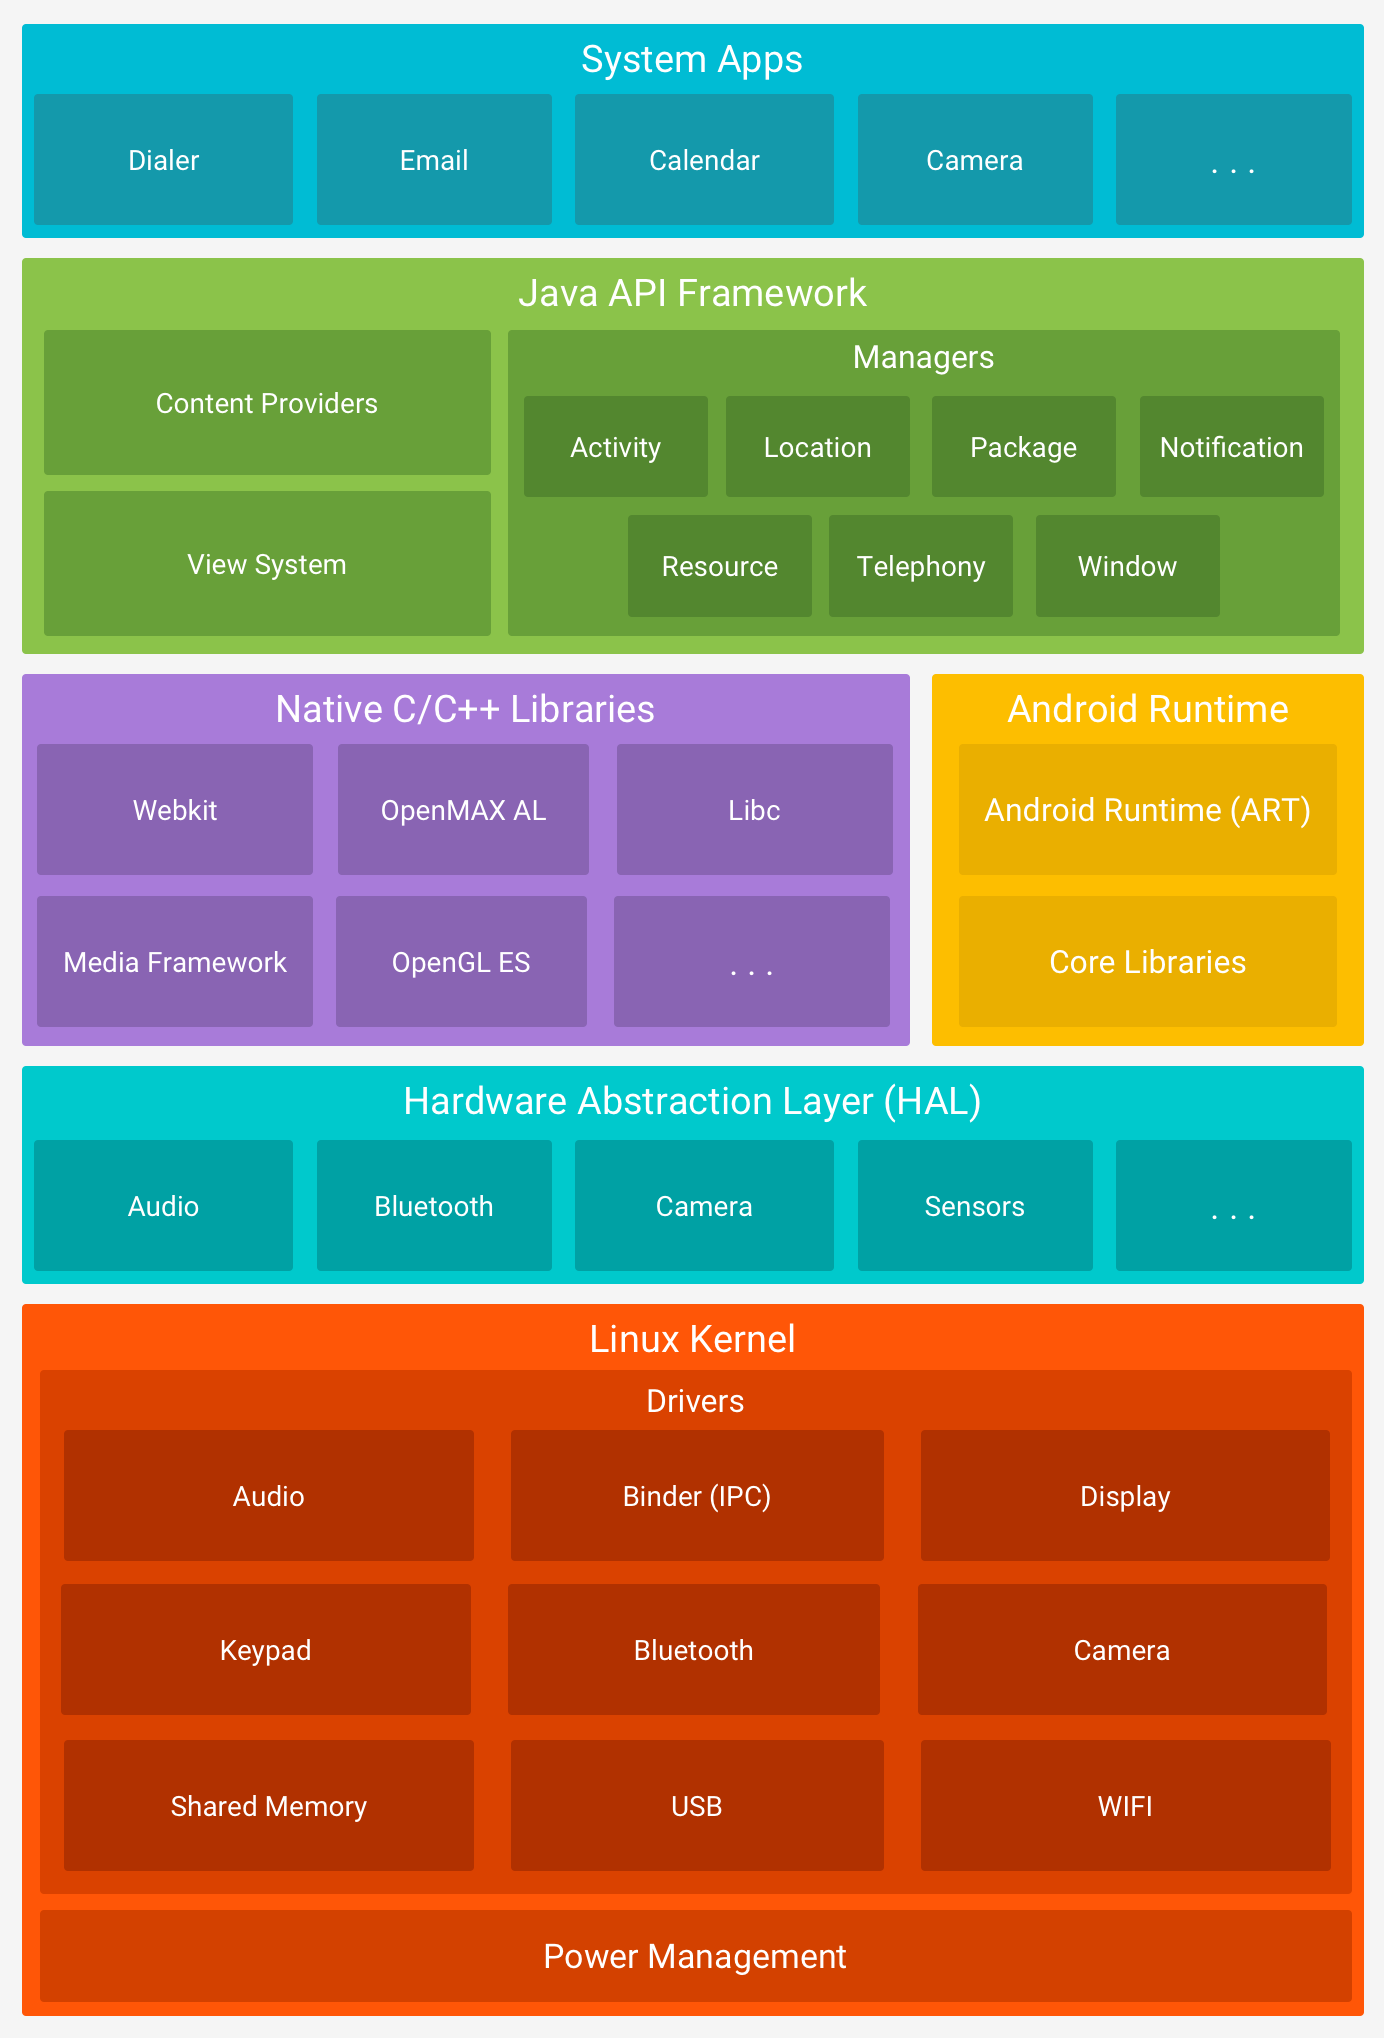
\includegraphics[scale=0.11]{immagini/android.png}
        \caption{Architettura di Android}
        \label{android}
      \end{figure}
    \newpage
    \subsection{Git e Bitbucket}
      Come \textit{software} di controllo di versione distribuito viene utilizzato Git.\\
      Attraverso l'utilizzo di Git è possibile gestire progetti anche molto complessi in modo efficiente, infatti perché consente a due o più persone di lavorare contemporaneamente sullo stesso file, senza perdita di consistenza, senza la necessità di collegamento di rete e senza conservare copie di backup in luoghi separati.\\
      L'azienda ha deciso di sfruttare, come \textit{hosting} per le proprie \textit{repository}, BitBucket in modo da facilitare la gestione del codice ed automatizzare alcune procedure.\\
      Infatti BitBucket integra il concetto di \textit{pipeline}, cioè una sequenza di \nameref{Task} che permette di eseguire script. In questo modo è possibile automatizzare i \textit{test} che verranno eseguiti ad ogni \textit{commit}.
      \begin{figure}[h]
        \centering
        
\includegraphics[scale=0.3]{immagini/bitbucket.png}
        \caption{Logo Bitbucket}
        \label{bit}
      \end{figure}
    \subsection{G Suite}
      È la soluzione per l'ufficio di Google e offre una gestione completa di email, \textit{editor} di testo, fogli di calcolo, calendario e archivio.\\
      Il principale vantaggio nell'utilizzarla è la possibilità di accedere ai dati in completa mobilità.\\
      I prodotti più utilizzati sono Drive per lo \textit{storage}, Docs per i documenti, Spreadsheet per i fogli di calcolo, Gmail per la gestione delle email. Include inoltre Hangouts che, come detto precedentemente viene utilizzato per le comunicazioni.
      \begin{figure}[h]
        \centering
        
\includegraphics[scale=0.2]{immagini/gsuite.png}
        \caption{Logo G suite con alcuni prodotti}
        \label{logog}
      \end{figure}
      \newpage
      \null
      \thispagestyle{empty}
      \newpage

  
\chapter{Presentazione dello stage}
  \section{Descrizione del progetto di stage}
    \subsection{Prodotto}
    \subsubsection*{ERA - Enterprise Remote Assistance}
      La mission di Vision Lab Apps è il miglioramento delle condizioni di lavoro tramite l'utilizzo della tecnologia, che sviluppa strumenti \textit{hardware} e \textit{software} sempre più innovativi.\\
      ERA (Enterprise Remote Assistance) nasce dall'idea di aumentare le capacità operative del personale del settore manifatturiero tramite l'utilizzo della realtà aumentata.\\
      Nello specifico l'azienda pensa di sfruttare la potenza dei Google Glass per fornire uno strumento per permettere di:
      \begin{itemize}
        \item ricevere istruzioni sulle attività da svolgere;
        \item eseguire passaggi e procedimenti operativi;
        \item condividere informazioni;
        \item offrire supporto in tempo reale.
      \end{itemize}
      Tutto questo permette di procedere attraverso flussi di lavoro, cercando informazioni e contenuti in tempo reale.\\
      Si può inoltre tenere traccia dello svolgimento delle attività, documentandone i passaggi cruciali attraverso la registrazione di foto e video passo passo che poi potranno essere condivisi per la formazione.\\
      Si ricerca anche la funzionalità di trasmettere video in diretta, in modo da fornire assistenza in tempo reale al personale non completamente specializzato nell'attività che sta eseguendo.
    \newpage
    \subsection{Tecnologie}
    \subsubsection*{Android}
      Il prototipo dell'applicazione è stato sviluppato in Android e questo permette lo \textit{streaming} video e audio su due dispositivi in cui è installata l'applicazione.
      \begin{figure}[h]
        \centering
        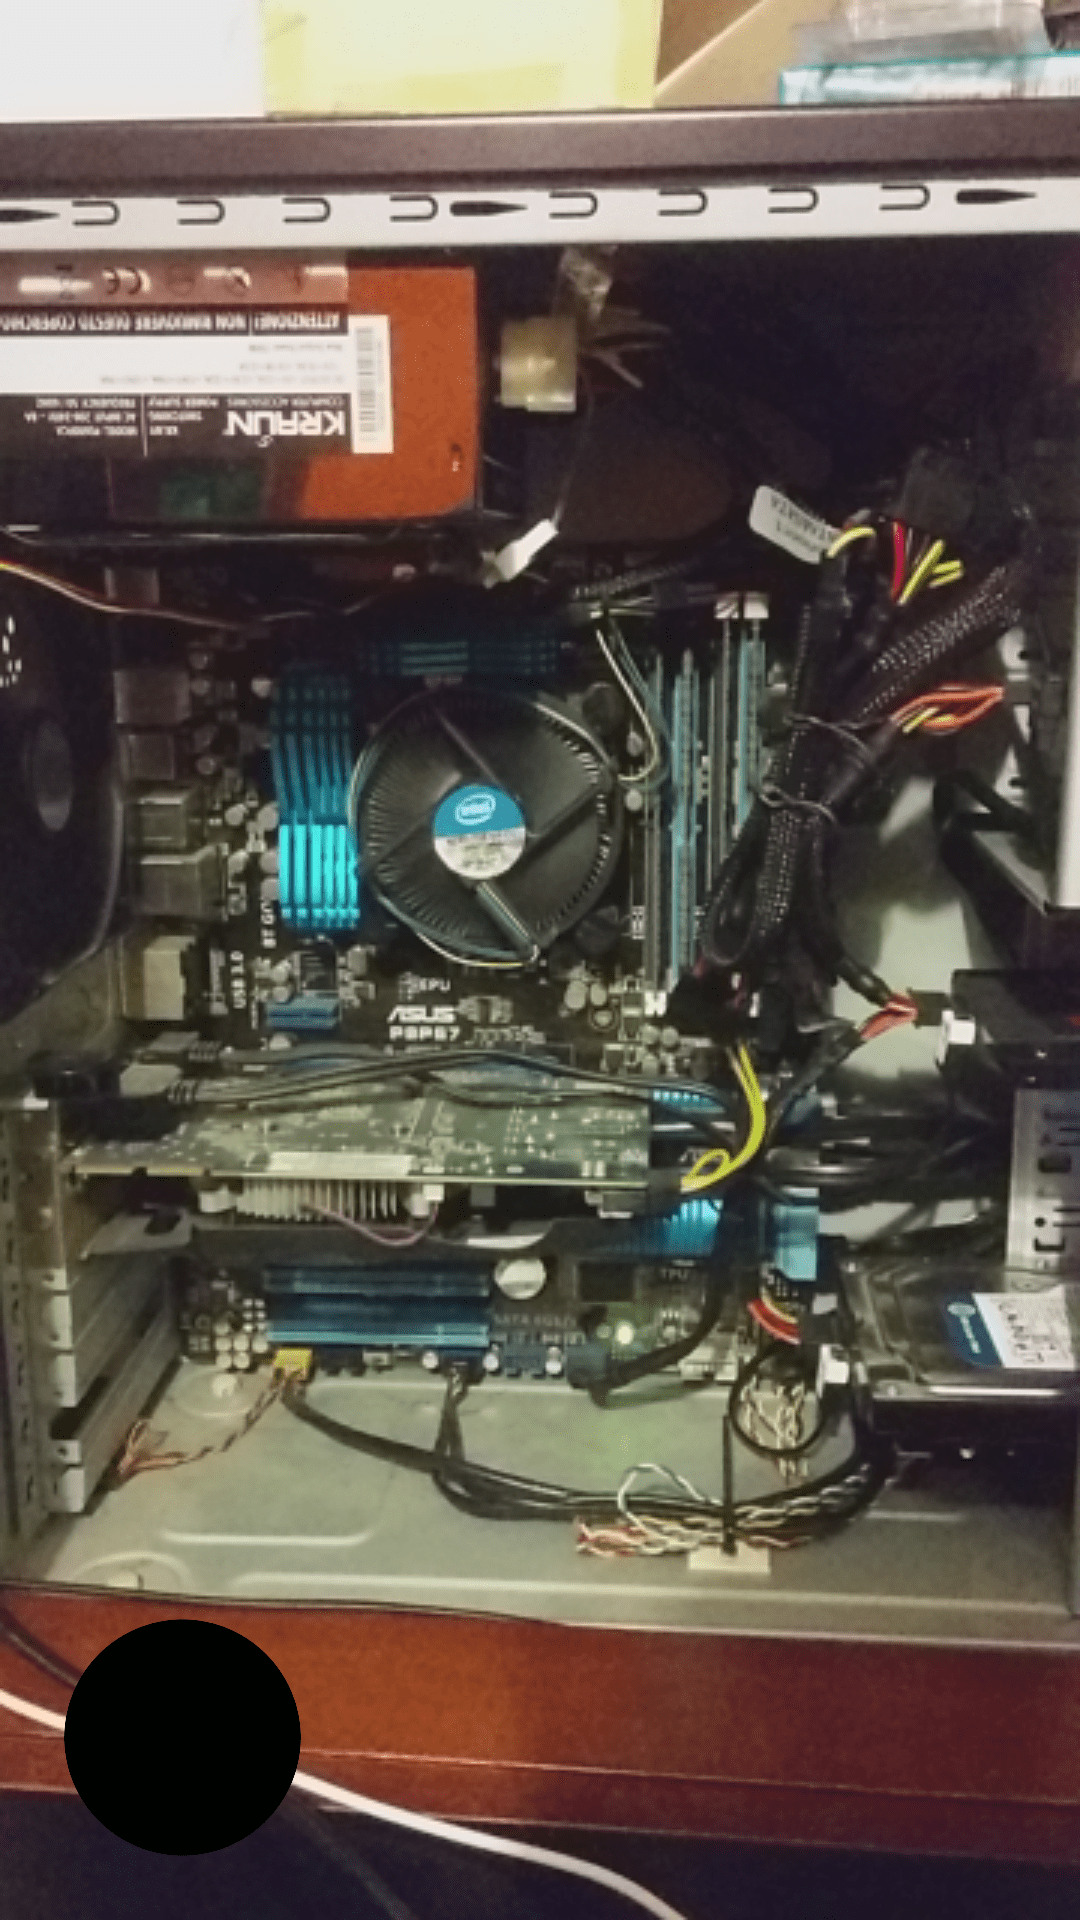
\includegraphics[width=180pt, height=320pt]{immagini/era.png}
        \caption{Streaming video su ERA}
        \label{era}
      \end{figure}
    \subsubsection*{Java}
      Per lo sviluppo del server per gestire l'autenticazione degli utenti ai vari canali, è stato sviluppato un prototipo di un'architettura client-server in Java, utilizzando il protocollo \nameref{TCP} tramite l'utilizzo di \nameref{Web}, ricercando una migliore soluzione in termini di latenza, throughput e complessità di implementazione.\\
      Lo \textit{standard} \nameref{Web} viene utilizzato per trasmettere stream di byte integrando però controlli di rete e sicurezza.\\
      Sono stati modellati, inoltre, gli utenti e nello specifico l'amministratore che può gestire i canali, controllando l'accesso ad utenti comuni.\\
      Tutto questo con una serie di controlli che permettono la gestione dei canali e dei messaggi che vengono mandati in questi stream.
    \subsubsection*{Firebase}
      In fase sperimentale è stato usato Firebase in quanto fornisce un \textit{database} e l'integrazione con dispositivi \textit{mobile}.\\
      Questo ha permesso lo sviluppo dell'applicazione Android ma anche della comunicazione con il server.
      \newpage
      \null
      \thispagestyle{empty}
      \newpage

  \chapter{Svolgimento dello stage}
  \section{Metodo di lavoro}
    Per tutta la durata dello stage sono stati seguiti i principi del modello \textit{Agile}, usato dall'azienda per lo sviluppo dei prodotti e la gestione dei progetti.
  \section{Attività preliminari}
    \subsection{Preparazione dell'ambiente di lavoro}
      \subsubsection{Sistema operativo}
        Il primo passo e stato l'installazione e configurazione di tutti gli strumenti necessari allo sviluppo del progetto.\\
        Come sistema operativo è stato scelto Linux Mint 18.2 denominato Sonya nella versione Cinnamon, noto ambiente grafico.\\
        Si basa su Ubuntu 16.04, un versione LTS, che quindi non richiede cambiamenti ai pacchetti fondamentali.
        \begin{figure}[h]
          \centering
          
\includegraphics[scale=0.1]{immagini/linuxmint.png}
          \caption{Logo Linux Mint}
          \label{logoMint}
        \end{figure}
      \subsubsection{IDE}
        Sono stati scelti due \nameref{IDE}: IntelliJ IDEA e Android Studio.\\\\
        IntelliJ IDEA è il punto di riferimento per quanto riguarda lo sviluppo in Java, in quanto permette di utilizzare molti automatismi che semplificano la codifica, come ad esempio un autocompletamento efficace, un debugger intuitivo e semplice da usare e che agevola il controllo del programma.\\\\
        Android Studio è invece l'\nameref{IDE} ufficiale per quanto riguarda la programmazione Android.\\\\
        Si basa sul \textit{software} di IntelliJ IDEA e quindi possiede tutte le sue caratteristiche, con l'aggiunta di altri strumenti che facilitano la programmazione in Android. Un esempio è l'emulatore virtuale che permette di eseguire l'applicazione sulla stessa macchina in cui è stato scritto, oppure la possibilità di caricare l'applicazione tramite USB direttamente nello smartphone.
        \begin{figure}[h]
          \centering
          
\includegraphics[scale=0.3]{immagini/ide.png}
          \caption{Logo IntelliJ IDEA e Android Studio}
          \label{logoIntellij}
        \end{figure}
      \subsubsection{Git}
      Per quanto riguarda il versionamento del codice, è stato utilizzato Git sfruttando l'\textit{hosting} offerto da Bitbucket, dove era presente il codice sorgente delle componenti già sviluppate dall'azienda.\\
      Si è optato di avvalersi di GitKraken, un \textit{software} che permette di eseguire le operazioni classiche di Git tramite un'interfaccia grafica.
      \begin{figure}[h]
        \centering
        
\includegraphics[scale=0.5]{immagini/gitkraken.png}
        \caption{Logo GitKraken}
        \label{logoKraken}
      \end{figure}
    \newpage
    \subsection{Formazione sulle componenti esistenti}
    Dopo aver predisposto l'ambiente di lavoro è cominciata la formazione sulle componenti già esistenti, che constano dell'applicazione Android e del server Java.\\\\
    L'applicazione Android, in sostanza, è costituita da una chat che dà la possibilità di effettuare lo \textit{streaming} audio e video, con un contatto presente nella rubrica dell'applicazione.\\
    Le sue varie funzionalità sono state spiegate da uno degli sviluppatori dell'applicazione, seguendo il codice sorgente per rendere più chiaro il perché delle scelte fatte.\\\\
    Per quanto riguarda il server Java l'azienda ha fornito il codice sorgente e la documentazione.
    \subsection{Studio individuale}
      \subsubsection{Applicazione Android}
        Dopo una rapida visione del codice con lo sviluppatore dell'applicazione, lo studio individuale è continuato ripercorrendo il codice sorgente e visionando la documentazione ufficiale di Android che, essendo ben scritta e molto chiara, ha contribuito ad una maggiore comprensione delle scelte.
      \subsubsection{Server Java}
        A causa del codice non molto commentato e della documentazione troppo caotica, il funzionamento del server Java non risultava molto chiaro; l'obiettivo è stato quello di migliorarlo.
      \newpage
      \subsubsection{Eclipse Vert.x}
        \begin{figure}[h]
          \centering
          
\includegraphics[scale=0.1]{immagini/Vertx.png}
          \caption{Logo Vert.x}
          \label{logoVertx}
        \end{figure}
        La ricerca di una soluzione per il server Java necessitava di un'alternativa che permettesse uno sviluppo più semplice, che però portasse anche a un miglioramento prestazionale.\\
        Alla fine la scelta è ricaduta su Eclipse Vert.x, un \nameref{Tool} per creare ed eseguire \nameref{RA} su una \nameref{JVM}.\\
        I punti di forza osservati durante lo studio sono:
        \begin{itemize}
          \item l'alta scalabilità: è basato su eventi e non è bloccante, consente infatti di gestire molta concorrenza utilizzando pochi thread;
          \item il fatto di essere poliglotta: si può usare questo \nameref{Tool} con vari linguaggi (Java, \nameref{JS}, \nameref{Groovy}, \nameref{Ruby}, \nameref{Scala}), infatti possiede delle \nameref{API} che in automatico permettono di utilizzare il linguaggio scelto andando a lavorare comunque su una \nameref{JVM};
          \item l'ottima documentazione: è presente infatti la spiegazione di tutti i metodi nei linguaggi citati precedentemente e sono presenti anche degli esempi di codice commentati e comprensibili.
        \end{itemize}
        All'interno di questo \nameref{Tool} sono presenti numerosi moduli che permettono di eseguire azioni che, utilizzando Java nativamente, risulterebbero più laboriose e quindi più predisposte ad errori.\\
        Per utilizzare il modulo che più ci interessa, basterà configurarlo correttamente per poterlo sfruttare da subito in semplicità.\\\\
        La caratteristica principale di questo \nameref{Tool} è l'Event Loop, il thread principale che permette di richiamare i gestori degli eventi appena questi arrivano.\\
        La regola fondamentale è non bloccare mai questo loop con costrutti come wait, sleep o attese di acquisizione di lock.\\
        La scalabilità viene gestita in automatico su un'architettura multi core: nel caso arrivassero troppe richieste ad un Event Loop, ne verrebbe istanziato uno aggiuntivo su un altro core e, automaticamente, le richieste in eccesso passerebbero al nuovo Event Loop istanziato.\\
        Un altro costrutto fondamentale è l'Event Bus che permette alle diverse parti di un'applicazione di comunicare tra loro, indipendentemente dal linguaggio in cui sono scritte.\\\\
        Vert.x, inoltre, fornisce un modello di implementazione e di concorrenza semplice e scalabile. Questo modello si chiama Verticle, fornisce metodi che in automatico utilizzano l'Event loop e comunicano tra loro tramite l'Event Bus.\\
        Queste funzionalità permettono di eseguire, in modo del tutto trasparente, tutti gli automatismi del \nameref{Tool} rendendo l'applicazione molto più reattiva.
        \begin{figure}[h]
          \centering
          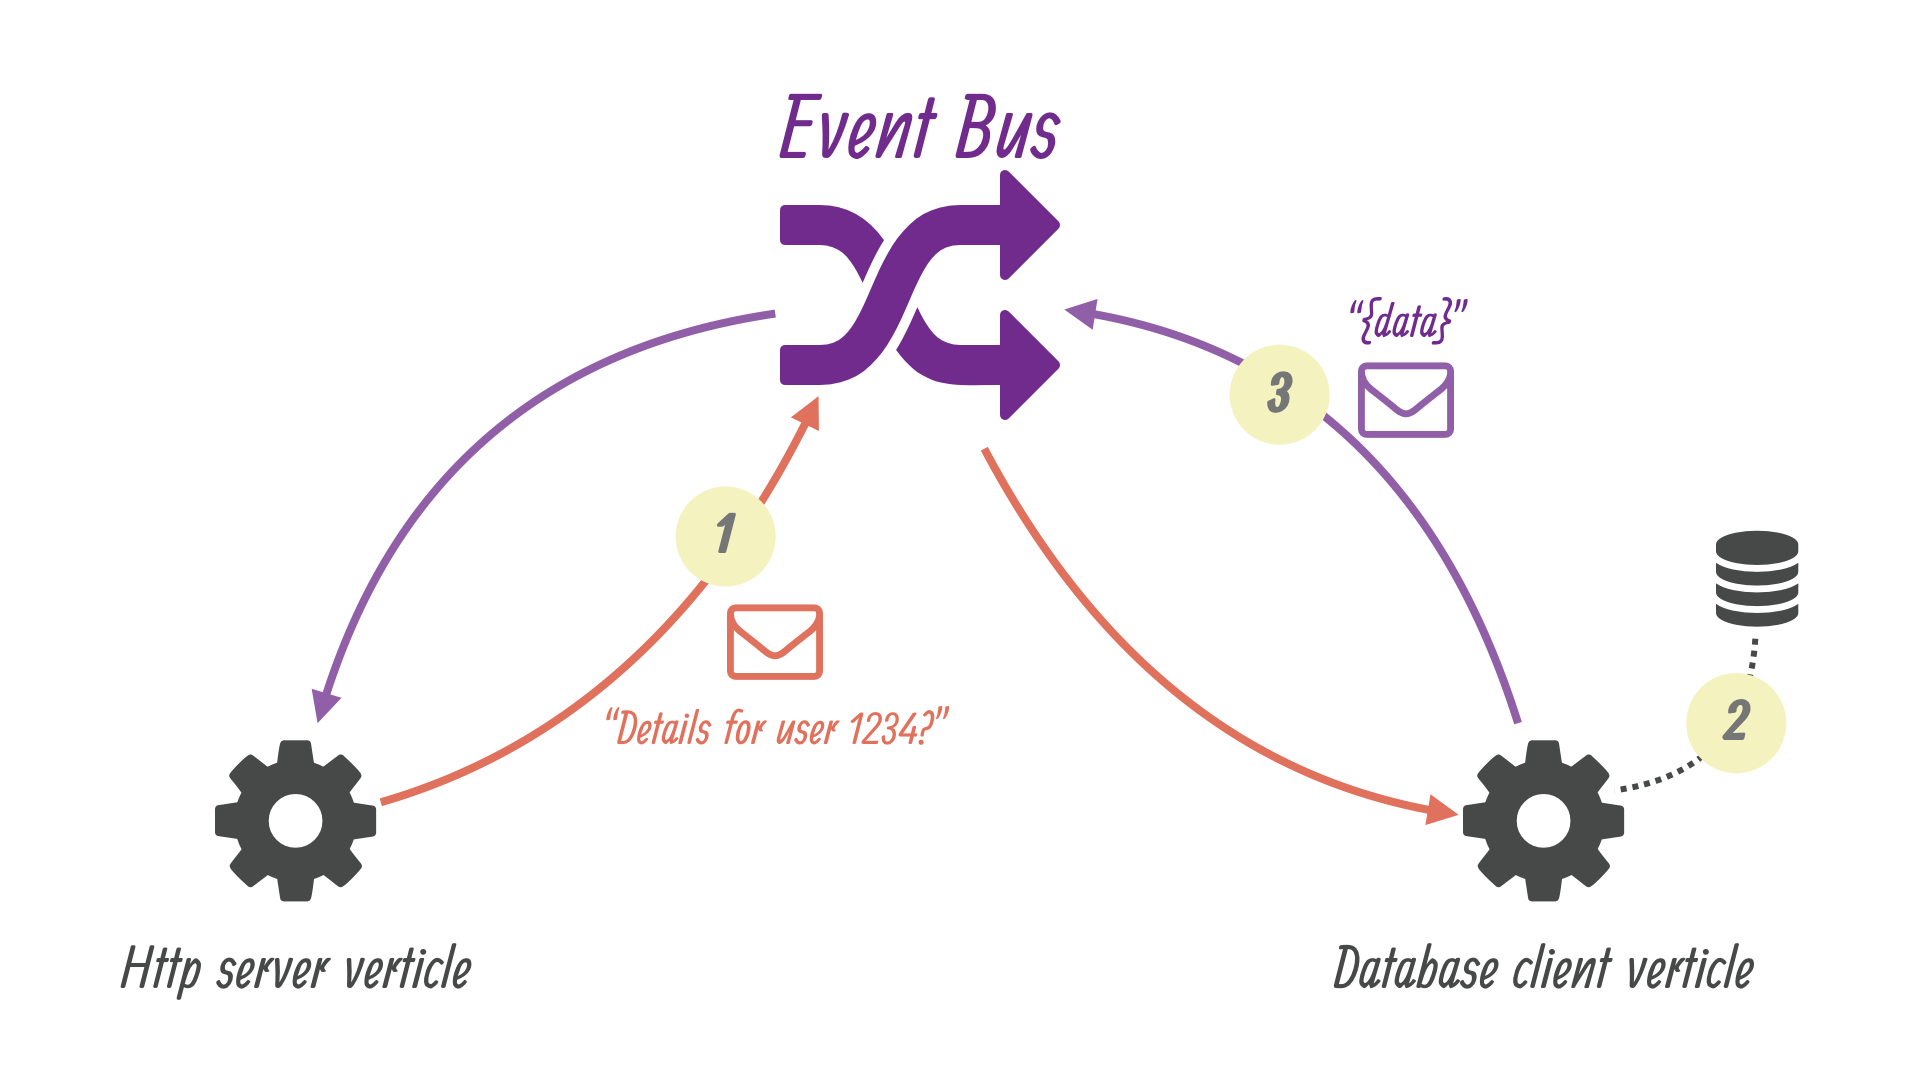
\includegraphics[scale=0.2]{immagini/event-bus.png}
          \caption{Esempio di utilizzo di due Verticle che comunicano tramite Event Bus per gestire una chiamata a database}
          \label{}
        \end{figure}
  \newpage
  \section{Sviluppo delle componenti}
    \subsection{Analisi dei requisiti}
      Le problematiche principali sono state riscontrate nel server Java quindi, in accordo con il tutor aziendale, è stato deciso di reimplementare questa componente utilizzando Vert.x.\\\\
      Lo scopo principale di questa componente è di permettere ad un utente con privilegi superiori di gestire un canale di comunicazione con uno o più utenti.\\
      In particolare deve essere possibile creare questo canale per permettere la comunicazione tra due tipi di utenti.\\
      Quindi, per ovvi motivi, deve consentire l'invio e la ricezione di messaggi e per questi deve essere possibile risalire a mittente e destinatario.\\\\
      C'è poi la necessità di discriminare tra le due tipologie di utenti che, avendo ruoli diversi, hanno anche funzionalità diverse.\\
      Deve essere presente un utente amministratore che può creare il canale di comunicazione, inviare messaggi, ricevere messaggi, limitare l'accesso ad alcuni utenti e infine chiudere il canale.\\
      Le modalità di accesso devono essere selettive, in modo da permettere all'amministratore un maggior controllo al fine di ridurre il carico di lavoro.\\\\
      L'altra tipologia di utente è quella base, cioè quella che può richiedere accesso ad un canale, inviare e ricevere messaggi nello stesso e infine abbandonarlo.\\\\
      Per ridurre l'astrazione il \textit{team} ha progettato, in parallelo, un'interfaccia grafica ed è stato richiesto, in modo facoltativo, di introdurla nell'architettura.\\
      In questo modo è possibile osservare i risultati effettivi delle funzionalità sviluppate.\\
      Un altro obiettivo opzionale è quello di integrare il sistema nell'applicazione Android, permettendo così l'effettiva unione dei due in un sistema più complesso e completo.\\
      Date le necessità descritte, si ottiene il seguente elenco dei requisiti:
      \begin{itemize}
        \item Obbligatori:
          \begin{itemize}
            \item implementazione di funzionalità che permettano di creare e gestire un canale di comunicazione;
            \item implementazione delle due tipologie di utenti distinguendo le modalità di uso del canale di comunicazione;
            \item implementazione di un sistema di permessi che permetta l'accesso solo ad utenti autorizzati.
          \end{itemize}
        \item Opzionali:
          \begin{itemize}
            \item integrazione dell'interfaccia grafica sviluppata dal \textit{team} all'interno del sistema, al fine di ridurre l'astrazione;
            \item integrazione della componente server con l'applicazione Android, in modo da creare un sistema più completo.
          \end{itemize}
      \end{itemize}
    \subsection{Progettazione}
      \subsubsection*{Canale di comunicazione}
        Nella versione precedente, il canale di comunicazione risultava di difficile comprensione e utilizzo in quanto eseguiva delle azioni considerate inutili.\\
        Si è deciso quindi di ridefinirlo e renderlo più semplice, sia di comprensione che di utilizzo.\\
        Un canale di comunicazione deve fare in modo di collegare due o più utenti, quindi in primo luogo deve essere possibile crearlo, individuarlo attraverso un identificativo e, infine, potervi accedere.\\
        Avrà quindi un identificativo che gli verrà assegnato alla creazione. È anche utile tenere una lista degli utenti che lo utilizzano in modo da semplificare poi la rimozione di uno di questi.\\
        Le funzionalità che deve offrire invece sono:
        \begin{itemize}
          \item creazione ed eliminazione;
          \item invio e ricezione di messaggi;
          \item la possibilità di rimuovere uno o più utenti dalla lista degli utilizzatori dello stesso.
        \end{itemize}
        Il concetto di messaggio viene modellato in modo molto basilare, con:
        \begin{itemize}
          \item mittente;
          \item destinatario;
          \item data e ora di invio;
          \item testo del messaggio.
        \end{itemize}
      \newpage
      \subsubsection*{Utenti}
        Un utente deve essere univoco, quindi deve avere un identificativo proprio e una password per ragioni di sicurezza, in modo da evitare usi indesiderati.\\
        Deve essere fornito di funzionalità base, quali:
        \begin{itemize}
          \item invio di messaggi attraverso il canale di comunicazione;
          \item chiusura della conversazione e dell'istanza di assistenza.
        \end{itemize}
        Ogni utente deve avere anche una tipologia, che può essere: amministratore o base. Questa distinzione è necessaria in quanto le due tipologie hanno funzioni diverse, in aggiunta a quelle di base.\\\\
        L'amministratore deve avere la possibilità di autorizzare uno o più utenti base ad accedere al canale di comunicazione.\\
        Deve anche essere possibile rimuovere una parte di utenti base che partecipano alla conversazione. Questo perché nel caso fosse stata completata l'assistenza per una parte di utenti, questi possono uscire da soli oppure devono essere rimossi, in modo da poter proseguire l'assistenza con la parte di utenti restante.\\\\
        L'utente base, invece, come funzionalità aggiuntiva presenta solo la possibilità di richiedere l'autorizzazione di accedere al canale. Questo meccanismo serve appunto a permettere all'utente base di cominciare a ricevere assistenza.
        \begin{figure}[h]
          \centering
          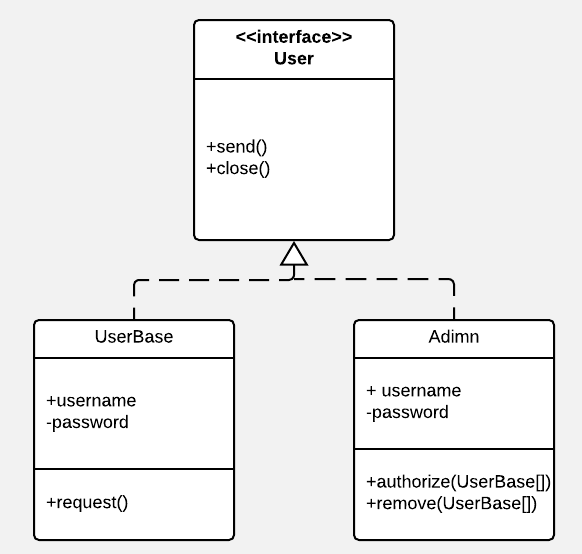
\includegraphics[scale=0.75]{immagini/user.png}
          \caption{Diagramma della classe User}
          \label{user}
        \end{figure}
      \subsubsection*{Sistema di autorizzazione}
        Deve essere possibile gestire l'accesso al canale di comunicazione. Questo verrà reso possibile sia lato amministratore sia lato utente base.\\\\
        Lato \textit{utente base} deve essere possibile effettuare una richiesta di assistenza, dalla quale segue l'autorizzazione da parte dell'amministratore. Questa richiesta viene resa possibile tramite l'invio di un messaggio contenente un testo con il tipo di assistenza che si necessita.\\\\
        Lato \textit{amministratore} deve essere possibile visualizzare le richieste effettuate dagli utenti base, l'autorizzazione a uno o più utenti ad accedere al canale di comunicazione e infine un'eventuale funzionalità di rimozione.\\
        La rimozione può essere effettuata in caso di errore oppure quando un determinato sottoinsieme di utenti non necessita di assistenza aggiuntiva.\\\\
        In questo modo è possibile gestire tutte le richieste simili in una sola volta, in modo da diminuire il carico di lavoro dell'amministratore.
      \subsubsection{Integrazione dell'interfaccia grafica}
        L'interfaccia grafica creata dal \textit{team} è composta da diverse componenti:
        \begin{itemize}
          \item struttura grafica della chat, che contiene tutte le parti di una classica chat quali:
          \begin{itemize}
            \item contenitore dei messaggi inviati;
            \item text area dove scrivere i messaggi da inviare;
            \item bottone per accedere al menù;
          \end{itemize}
          \item log in che comprende due campi dove inserire l'identificativo dell'utente e la sua password per poter accedere al sistema;
          \item menù amministratore che contiene:
          \begin{itemize}
            \item visione delle richieste;
            \item autorizzazione lista utenti;
            \item rimozione utenti dalla conversazione;
          \end{itemize}
          \item menù utente base, contenente un link a una pagina in cui è presente un form per inviare la richiesta di assistenza.
        \end{itemize}
        Entrambi i menù contengono inoltre un bottone per effettuare l'operazione di log out.\\\\
        Tutte queste componenti grafiche devono essere integrate con il sistema in modo da rendere il sistema sottostante più concreto e visibile.
        \begin{figure}[h]
          \centering
          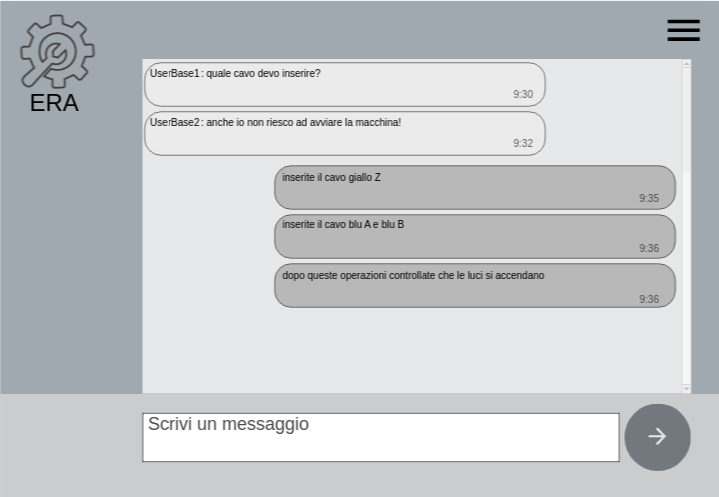
\includegraphics[scale=0.5]{immagini/chat.png}
          \caption{Esempio conversazione}
          \label{chat}
        \end{figure}
    \subsection{Implementazione}
      \subsubsection*{Canale di comunicazione}
        Come prima operazione, è stata definita la struttura JSON del messaggio.
        \begin{codice_json}[]
          {
            "sender": string,
            "receiver": string,
            "date": [
              {
                "year": number,
                "month": number,
                "day": number,
                "hours": number,
                "minutes": number
              }
            ],
            "text": string
          }
        \end{codice_json}
        \begin{description}
          \item[sender]: mittente, variabile di tipo string;
          \item[receiver]: destinatario, variabile di tipo string;
          \item[date]: data, array di variabili number contenenti anno, mese, giorno, ore, minuti;
          \item[text]: testo del messaggio, variabile di tipo string.
        \end{description}
        Successivamente come canale di comunicazione è stato scelto l'Event Bus, un oggetto fornito da Vert.x che fornisce appunto un sistema di trasmissione dati fra istanze di Vert.x.\\
        La caratteristica principale di questo bus è il fatto di essere \textit{distribuito} di default, senza la necessità di usare meccanismi come \nameref{RMI}.\\
        L'unica cosa che viene richiesta è che, alla creazione dell'Event Bus, questo venga configurato. Segue del codice di esempio.
        \begin{codice_java}
          VertxOptions options = new VertxOptions()
            .setEventBusOptions(new EventBusOptions()
            .setClusterPublicHost("IDcanale")
            ); /*tramite questo codice viene fornito l'identificativo al canale che potra' quindi essere riconosciuto anche esternamente*/
            Vertx.clusteredVertx(options, res -> {
              if (res.succeeded()) {
                Vertx vertx = res.result();
                EventBus eventBus = vertx.eventBus(); //in questo momento viene creato effettivamente l'EventBus con le impostazioni scritte precedentemente
                System.out.println("Success:" + eventBus);
              }
              else {
                System.out.println("Failed:" + res.cause());
              }
            });
        \end{codice_java}
        Le funzionalità esposte dal tipo Channel, che utilizza l'EventBus, sono state implementate utilizzando alcuni metodi propri di EventBus.
        \begin{itemize}
          \item\textbf{create(UserBase[] list):} crea l'EventBus configurandolo e aggiungendo l'amministratore e una lista di utenti base;
          \item\textbf{send(JsonObject message):} utilizza il metodo \verb+send(String address, Object message)+ di EventBus per inviare il messaggio;
          \item\textbf{remove(UserBase[] list)}: utilizza il metodo \verb+removeInterceptor(Handler<SendContext>+\linebreak \verb+interceptor)+ per rimuovere utenti base dal canale di comunicazione;
          \item\textbf{authorize(UserBase[] list)}: utilizza il metodo \verb+addInterceptor(Handler<SendContext> +\linebreak \verb+ interceptor)+ per aggiungere utenti base al canale di comunicazione;
          \item\textbf{destroy()}: utilizza \verb+close(Handler<AsyncResult<Void>> completionHandler)+ per chiudere il canale di comunicazione e rilasciare le risorse.
        \end{itemize}
      \subsubsection*{Utenti}
        Dovendo modellare due tipologie di utenti che condividono delle azioni, è stata creata un'interafaccia, User, contenente le funzionalità comuni di invio del messaggio e chiusura della conversazione.\\
        Successivamente sono state modellate altre due classi che implementano User, per creare l'amministratore, Admin, e l'utente base, UserBase.\\\\
        UserBase, oltre a implementare i metodi ereditati da User, ha anche un altro metodo che permette di effettuare la richiesta di assistenza, inviando un messaggio inserito in un \nameref{JSON}, all'amministratore.\\\\
        Admin alla stessa maniera, implementa i metodi ereditati da User, ma aggiunge due ulteriori metodi: uno che permette di autorizzare un insieme di UserBase e uno che permette la rimozione di un utente dalla conversazione.\\
        \begin{codice_java}
          public interface User{
            public void send(JsonObject);
            public void close();
          }
          public class UserBase implements User{
            public String username;
            private String password;
            public void request(){
              //corpo del metodo
            }
            //ridefinizioni dei metodi di User
          }
          public class Admin implements User{
            public String username;
            private String password;
            public void authorize(UserBase[]){
              //corpo del metodo
            }
            public void remove(UserBase[]){
              //corpo del metodo
            }
            //ridefinizioni dei metodi di User
          }
        \end{codice_java}
        Tutti questi metodi sono delle chiamate a metodo di Channel.

      \newpage
      \subsubsection*{Sistema di autorizzazione}
        Per gestire il sistema di autorizzazione è stato usato l'automatismo di default fornito da Vert.x.\\
        UserBase utilizza il metodo \verb+request()+ ed invia un primo messaggio, contenuto in un \nameref{JSON}, per indicare la richiesta di assistenza.\\
        Questo notifica ad Admin la volontà di un UserBase di ricevere assistenza.\\
        Quando arriva questa richiesta l'Admin può confermarla inserendo l'utente richiedente con l'apposito metodo \verb+authorize(UserBase[])+ nel canale di comunicazione.\\
        Il metodo, se viene chiamato per la prima volta, utilizza il metodo \verb+create(UserBase[] list)+ di Channel inserendo l'Admin e la lista di UserBase che è stata passata come argomento.\\

      \subsubsection*{Integrazione interfaccia grafica}
        Per integrare l'interfaccia grafica, fornita dal \textit{team}, scritta in \nameref{HTML}, \nameref{CSS} e \nameref{JS}, sono stati creati due Verticle, che permettono inoltre di gestire le varie componenti appena definite.\\\\
        Lato server è stato creato un Verticle, modello consigliato nell'utilizzo di Vert.x, per avviare un server \nameref{HTTP} e un server \nameref{Web}.\\
        Vert.x ha reso tutto questo molto semplice in quanto per creare il server \nameref{HTTP} è bastata una semplice chiamata a metodo:\\\\
        \verb|VertX.createHttpServer().requestHandler(httpRouteMatcher).listen(8080,"localhost");|\\\\
        Per quanto riguarda invece il server \nameref{Web}, deve inizialmente rifiutare tutte le connessioni che non possiedono l'autorizzazione per accedere al canale di comunicazione.\\
        In caso si possegga tale autorizzazione sarà possibile accedere alla conversazione.\\
        Questa si identifica nell'EventBus che permetterà, tramite l'utilizzo dei metodi citati precedentemente, la comunicazione tra amministratore e utente base.\\\\
        \newpage
        Lato \textit{client} invece è stata inserita l'interfaccia grafica fornita dal \textit{team}, aggiungendo delle funzioni \nameref{JS} per permettere le funzionalità in base al tipo di utente.\\
        Questa implementazione gestisce l'invio dei messaggi attraverso l'EventBus, la chiusura della chat e l'autorizzazione da parte dell'amministratore di utenti.\\
        Segue l'esempio del codice che permette l'invio di un messaggio.\\
        \begin{figure}[h]
          \centering
          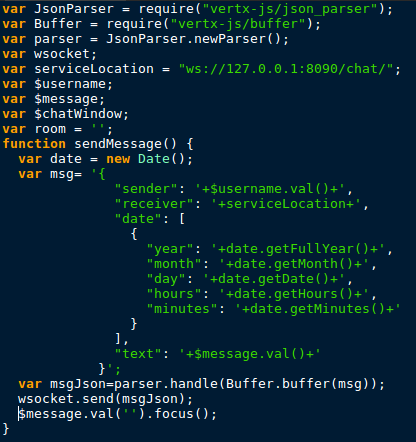
\includegraphics[scale=0.5]{immagini/sendJS.png}
          \caption{Codice per l'invio di messaggi}
          \label{cod}
        \end{figure}
  \newpage
  \section{Qualifica}
    \subsection{Verifica}
      La verifica di un prodotto è l'insieme delle operazioni che garantiscono la qualità e il rispetto delle specifiche.
      \subsubsection{Analisi statica}
        L'analisi statica consiste di \textit{test} che vengono eseguiti sul prodotto senza compilare ed eseguire codice.\\
        Questo tipo di analisi è stata delegata all'\nameref{IDE} utilizzato, in quanto fornisce strumenti di controllo di sintassi e suggerimenti sul completamento automatico.
      \subsubsection{Analisi dinamica}
        L'analisi dinamica è l'insieme delle operazioni di controllo che vengono fatte sul codice compilato ed eseguito.\\
        Per creare i \textit{test} è stato usato il modulo di Vert.x che permette di eseguirli in modo asincrono. Questo modulo utilizza delle componenti di framework come JUnit.
        Successivamente sono stati eseguiti in modo automatico, creando una \textit{pipeline} su Bitbucket.
      \subsubsection{Test}
        Vert.x permette, con il suo modulo, di creare test di unità e unirli per andare a generare una suite di test.\\
        Sono stati quindi definiti test di unità per tutte le singole componenti del sistema.\\
        Questi sono stati successivamente uniti per formare i test di integrazione che testassero il corretto funzionamento delle comunicazioni.
    \subsection{Validazione}
      La validazione di un prodotto consiste nel controllare che tutti i requisiti vengano effettivamente soddisfatti.
      \subsubsection{Validazione interna}
        Dato che il prodotto è ancora in via di sviluppo e destinato ad essere una componente di una piattaforma più grande, la sua validazione è stata interna.\\
        Sono stati eseguiti nuovamente tutti i \textit{test} e le simulazioni; infine come prova finale il tutor aziendale e un altro componente del \textit{team} hanno provato a comunicare tra di loro utilizzando il prodotto.
  \section{Analisi dei principali problemi}
    \subsection{Utilizzo Vert.x}
      Essendo tutto il progetto basato sull'utilizzo di Vert.x, lo studio di questo \nameref{Tool} ha portato a dei problemi.\\
      Questo perché presenta un insieme molto grande di moduli e quindi ha richiesto una mole di studio per comprendere appieno quali effettivamente bisognava usare.\\
      Tuttavia, seguendo la documentazione e visionando numerosi esempi, è stato possibile  restringere il campo d'azione e trovare e poi utilizzare i moduli che risultavano più corretti.
    \subsection{Metodo Agile}
      Inizialmente seguire il metodo \textit{Agile} è stato difficile, in quanto il tutor era spesso fuori sede o comunque concentrato su altri progetti.\\
      Tuttavia era comunque presente su i canali di comunicazione e rispondeva in tempi brevi.\\
      Una migliore pianificazione probabilmente avrebbe permesso di proseguire in modo più fluente il lavoro.
      \newpage
      \null
      \thispagestyle{empty}

  \cleardoublepage
\chapter{Conclusioni}
  \section{Obiettivi raggiunti}
    \subsection{Funzionalità componenti sviluppate}
    Al termine del periodo di stage sono stati raggiunti tutti i requisiti obbligatori e parte di quelli opzionali.\\
    In particolare:
    \begin{itemize}
      \item è stata ridefinita l'architettura server, gestendo in modo opportuno il canale di comunicazione e gli utenti lato amministratore;
      \item è stato reimplementato il sistema di permessi in modo da concedere a più utenti di accedere alla conversazione;
      \item è stata integrata nell'architettura l'interfaccia grafica, in modo da fornire una visione delle funzionalità disponibili.
    \end{itemize}
    \subsection{Sviluppi futuri}
      Durante lo sviluppo del progetto sono nate nuove idee riguardo alcune funzionalità da implementare.\\
      Una di queste è di fornire degli strumenti che manipolino lo streaming video in modo da permettere il tracciamento e l'evidenziazione di alcune parti di un macchinario che necessitano di assistenza.\\
      Questo permetterebbe di mostrare in modo più preciso uno step di un procedimento più o meno complicato, rendendo l'assistenza più efficiente e proficua.\\\\
      Un'altra opzione è quella di unire l'applicazione Android con il sistema sviluppato che, a causa del poco tempo rimasto, non è stato possibile fare.\\
      Bisognerà capire quanto difficile possa risultare la modifica dell'applicazione Android per integrare i tipi e i metodi che sono stati definiti per il sistema che è stato sviluppato.
  \section{Obiettivi personali}
    \subsection{Risultati ottenuti}
      Uno degli obiettivi che mi ero fissato prima di cominciare lo stage era di imparare qualcosa di nuovo, che mi portasse ad ampliare le mie conoscenze in un ambito che sta prendendo piede e che mi interessa.\\
      Questo obiettivo è stato raggiunto perché, anche se ho utilizzato una tecnologia già conosciuta, mi sono reso conto di non conoscerla così bene e di quanti altri modi ci fossero per poterla utilizzare.\\
      Inoltre il campo della realtà virtuale mi sta appassionando molto e, confrontandomi con persone che si intendono di più dell'argomento, mi permette di conoscere opinioni e idee che sono diverse dalla mia.
    \subsection{Valutazione personale}
      Inizialmente è stato difficile perché essendo la prima esperienza lavorativa di questo calibro, non ero completamente preparato a questa mole di lavoro.\\
      Tuttavia mi sono dovuto subito mettere in gioco, per studiare, analizzare le componenti già sviluppate e reimplementarle e alla fine sono soddisfatto del livello che ha raggiunto il progetto.\\
      Sono anche soddisfatto di non aver avuto problemi ad integrarmi nel team, dove ho trovato persone competenti e molto disponibili.\\\\
      Infine posso dire di essere orgoglioso di aver lavorato in un'azienda che si sta sviluppando molto e, anche se ha incontrato diversi problemi in passato, non ha mai perso l'entusiasmo e la voglia di mettersi in gioco.
\vfill
\newpage
\null
\thispagestyle{empty}

  \addcontentsline{toc}{chapter}{Glossario}
\markboth{Glossario}{Glossario}
\chapter*{Glossario}
    \subsubsection{\label{API}API}
      Acronimo di Application Programming Interface. Indica un insieme di procedure disponibili al programmatore, raggruppate a formare un set di strumenti specifici per espletare un determinato compito in un programma. La finalità è raggiungere il riuso del codice, tramite l'ottenimento di un'astrazione a più alto livello.
    \subsubsection{\label{CSS}CSS}
      Acronimo di Cascading Style Sheets. Linguaggio usato per la formattazione di documenti HTML. La sua introduzione si è resa necessaria per permettere una programmazione più chiara e semplice da utilizzare, tramite la separazione dei contenuti dalla loro formattazione.
    \subsubsection{\label{Groovy}Groovy}
      Linguaggio di programmazione ad oggetti per la piattaforma Java, alternativo al linguaggio Java. La sua sintassi è molto simile a quella di Java, infatti permette di interagire in modo trasparente con altro codice Java.
    \subsubsection{\label{HTML}HTML}
      Acronimo di HyperText Markup Language. È un linguaggio di markup che ha come scopo quello di gestire i contenuti associandone o specificandone allo stesso tempo il layout, per realizzare una pagina web, tramite l'utilizzo di tag diversi.
    \subsubsection{\label{HTTP}HTTP}
      Acronimo di HyperText Transfert Protocolo. È un protocollo a livello applicativo usato come sistema principale per la trasmissione di informazione nel web.
    \subsubsection{\label{IDE}IDE}
      Acronimo di Integrated Development Environment. È un software che aiuta i programmatori nella scrittura del codice sorgente. Fornisce strumenti e funzionalità di supporto alla fase di sviluppo e debugging, oltre che a segnalare errori di sintassi del codice durante la fase di scrittura.
    \subsubsection{\label{IoT}IoT}
      Acronimo di Internet of Things. Si riferisce all'estensione di Internet ad oggetti comuni, in modo che diventino più intelligenti. Questo porta a comunicare dati su sé stessi e sul mondo che li circonda e allo stesso tempo di accedere a informazioni nella rete.
    \subsubsection{\label{Java}Java}
      È un linguaggio di programmazione ad alto livello, orientato agli oggetti e a tipizzazione statica, progettato per essere il più possibile indipendente dalla piattaforma di esecuzione.
    \subsubsection{\label{JS}JavaScript}
      È un linguaggio di scripting orientato agli oggetti e agli eventi. Viene utilizzato nella programmazione web lato client per la creazione di effetti che scatenano funzioni invocate da eventi, a loro volta innescati dall'utente. Viene utilizzato anche per creare app per più sistemi operativi.
    \subsubsection{\label{JSON}JSON}
      Formato adatto allo scambio di dati tra applicazioni client-server. Si basta su un sottoinsieme di JavaScript ma ne è indipendente.
    \subsubsection{\label{JVM}JVM}
      Acronimo di Java Virtual Machine. È la componente della piattaforma Java che esegue i programmi che sono stati tradotti in bytecode dopo una compilazione.
    \subsubsection{\label{PMI}PMI}
      Acronimo di Piccole e Medie Imprese.
    \subsubsection{\label{PM}Project Manager}
      È il responsabile dell'organizzazione dei processi e della loro pianificazione all'interno di un progetto.
    \subsubsection{\label{RA}Reactive Application}
      È un tipo di programma che segue i principi descritti nel Reactive Manifesto, che dà le indicazioni per seguire il paradigma di programmazione Reactive.
    \subsubsection{\label{RMI}RMI}
      Acronimo di Remote Method Invocation. È una tecnologia che, utilizzata nel contesto del linguaggio di programmazione Java, consente a processi Java distribuiti di comunicare attraverso una rete.
    \subsubsection{\label{Ruby}Ruby}
      È un linguaggio di programmazione completamente ad oggetti. Si differenzia dal C++ per essere molto più dinamico, infatti è possibile aggiungere o modificare metodi a runtime. Un'altra particolarità è che il suo tipo non è definito dalla classe che lo istanzia, ma dall'insieme dei metodi che possiede.
    \subsubsection{\label{Scala}Scala}
      È un linguaggio di programmazione di tipo general-purpose multiparadigma che integra le caratteristiche sia dei linguaggi orientati agli oggetti che dei linguaggi funzionali.
    \subsubsection{\label{Sprint}sprint}
      Periodo temporale in cui devono essere portati a termine dei task.
    \subsubsection{\label{Task}task}
      È un compito da portare a termine. Richiede poche ore di lavoro e può essere preso in carico da una sola persona.
    \subsubsection{\label{Tool}toolkit}
      È un insieme di strumenti software di base per facilitare e uniformare lo sviluppo di applicazioni più complesse.
    \subsubsection{\label{TCP}TCP}
      Acronimo di Transmission Controll Protocol. È un protocollo di rete a pacchetto di livello trasporto che si occupa di controllo trasmissione. Questo protocollo rende affidabile la comunicazione dati in rete tra mittente e destinatario.
    \subsubsection{\label{Wear}wearable}
      È un dispositivo elettronico indossabile o impiantabile. In generale offrono funzionalità di notifica legate agli smartphone oppure presentano dei sensori. Questo tipo di dispositivi è un esempio di dispositivo IoT.
    \subsubsection{\label{Web}WebSocket}
      È una tecnologia web che fornisce canali di comunicazione full-duplex attraverso una singola connessione TCP.
      \newpage
      \null
      \thispagestyle{empty}
      

  \addcontentsline{toc}{chapter}{Sitografia}
\markboth{Sitografia}{Sitografia}
\chapter*{Sitografia}
\begin{itemize}
  \item Vision Lab Apps sito ufficiale \\ \url{http://www.visionlabapps.com/}
  \item Eclipse Vert.x \\ \url{http://vertx.io/}
  \item Eclipse Vert.x documentazione del core \\ \url{http://vertx.io/docs/vertx-core/java/}
  \item Eclipse Vert.x esempi del core \\ \url{https://github.com/vert-x3/vertx-examples/tree/master/core-examples}
  \item Jenkov tutorial di Vert.x \\ \url{http://tutorials.jenkov.com/vert.x/index.html}
  \item Git \\ \url{https://git-scm.com/}
  \item Bitbucket \\ \url{https://bitbucket.org/product}
  \item Reactive Manifesto \\ \url{https://www.reactivemanifesto.org/}
  \item GitKraken \\ \url{https://www.gitkraken.com/}
  \item IntelliJ IDEA \\ \url{https://www.jetbrains.com/idea/}
  \item Android \\ \url{https://www.android.com/}
  \item Android Studio \\ \url{https://developer.android.com/studio/index.html}
  \item Android documentazione API \\ \url{https://developer.android.com/guide/index.html}
  \item Linux Mint \\ \url{https://linuxmint.com/}
\end{itemize}

\end{document}
